%!TEX root = handout.tex

%%%%%%%%%%%%%%%%%%%%%%%%%%%%%%%%%%%%%%%%%%%%%%%%%%%%%%%%%%%%%%%%%%%%%%%%%%%%%%%%
\section{A basic KNIME Workflow}

This section will guide you through the creation of a simple KNIME workflow. We will read in a file, visualize its contents and transform the data in multiple ways. Additionally we cluster the data and learn a simple machine learning model on it.

\subsection{Creating a new Workflow}

Either go to \menu{File > New...} in the menu or right-click in your workflow repository and click \menu{New KNIME Workflow...}. In the window that is opened, type the name of the workflow you want to create. Optionally you can also change the place where the workflow is stored in your workflow repository. Click \menu{Finish} on the bottom right to create and open the workflow.

\subsection{Reading Data}

To search for a specific node in the node repository, just start typing its name in the search box. To read in a file using the popular File Reader node, type ''File Reader'' and drag the node from the repository onto your workspace.

\begin{figure}[h]
\centering
\includegraphics[width=0.59\textwidth]{graphics/knime_basics/new_node}
\caption{Adding a node from the node repository to the the workspace.}
\label{fig:new_node}
\end{figure}

You will find that the traffic light under the node is red and a warning symbol is shown. The red traffic light means that the node needs to be configured before being executed. When you hover with the mouse pointer over the warning symbol, it displays the message ''No settings available". To configure the node, double-click on it or right-click and select \menu{Configure...}.

\begin{figure}[h]
\centering
\includegraphics[width=0.59\textwidth]{graphics/knime_basics/config}
\caption{Top part of the configuration dialog of the File Reader node.}
\label{fig:config}
\end{figure}

The configuration dialog of the File Reader node allows you to specify the location of a text file containing a data table. It can read files from various sources, including HTTP, FTP and the local filesystem. For this tutorial, we will load the data from the UCI Machine Learning Repository. Enter the following URL into the textbox: \url{http://archive.ics.uci.edu/ml/machine-learning-databases/iris/iris.data}. The URL points to a data set about different types of iris flower data. Press the ENTER key on your keyboard to let KNIME inspect the file. If that takes too long, you can press the \menu{Quick Scan} button in the bottom half of the window so KNIME does not inspect the whole file. After the inspection is done, you see a preview of the data in the bottom half of the configuration window. Click \menu{OK} to close the dialog. You will notice that the warning side is gone and that the traffic light has switched to yellow, which means that the node is ready to be executed. Right-click on the node and then click on \menu{Execute} and notice how the traffic light first turns into a progress bar and then green. This means that it is finished and the result of the node's operation is available at the output port.

\note{Of course you can also load data from other sources. You find them in the node repository under \menu{IO > Read}.
It is also possible to read data from various databases such as MySQL, SQLite and Postgres.}

\subsection{Inspecting Output Data}

We now want to have a look at the data we just loaded with the File Reader node. Right-click on the node and then click on \menu{File Table} at the bottom of the context menu. All output ports of a node have an entry in this menu. You can find out an output port's name by hovering over it with the mouse. Once you click on the entry for the output port, a window with a data table is opened. You can click on a column to sort the table. Close the dialog to continue with the tutorial.

\subsection{Data Transformations}

\subsubsection{Column Renaming}
As we have seen in the data table view, our columns are just named Col0 to Col4. Let's give them proper names. Search for ''Column Rename'' in the node repository and drag the node onto the workspace, behind the File Reader node. To let data flow from the File Reader to the Column Rename, you have to connect the output port of the first with the input port of the latter. To do that, click and hold with the mouse onto the output port, then drag a line to the input port. Release the mouse when it is over the black triangle pointing towards the Column Rename node. However, the traffic light of the node is still red because we need to configure it. Double-click on it to open the configuration dialog.

\begin{figure}[h]
\centering
\includegraphics[width=0.59\textwidth]{graphics/knime_basics/connect}
\caption{Connecting a node to the output of another node.}
\label{fig:connect}
\end{figure}

On the left side, you see a list of the columns currently available in the table at the input port. Double-click on the column with the name ''Col4'' to change its name. It appears on the right side of the dialog and by clicking first onto the checkbox labeled ''Change'' you enable the naming text field. Please rename the column to ''class'' and close the dialog by clicking \menu{OK}. Make sure that the traffic light is yellow and then execute the node.

\subsubsection{Normalization}
For further analysis, we want to make sure that all the numeric columns are in the range from 0 to 1. To do so, we need the ''Normalizer'' node. Search for it in the node repository, add it and connect it to the output of the Column Rename node. You will notice that the traffic light is not red and the warning sign informs you that by default all numeric columns are normalized from 0 to 1. This means we do not have to configure the node. You can simply execute it without opening the configuration dialog.

\note{Some other useful data transformation nodes are the Binner, Row Filter, Column Filter, GroupBy and Joiner}

\subsection{Visualization}

\subsubsection{The Scatter Plot}

Now that we have the data in the format we want, we can visualize it. Search for ''Scatter Plot'' in the node repository and connect the plot to the top output of the Normalizer node. Execute the new node and then right-click on it. Now select \menu{View: Scatter Plot} from the context menu. What you see is a 2D representation of your data, with the x- and y-axes corresponding to a column in your table. Click on the tab ''Column Selection'' at the bottom to change the columns you want to display.

\begin{figure}[h]
\centering
\includegraphics[width=0.59\textwidth]{graphics/knime_basics/scatter}
\caption{A KNIME scatter plot view of the Iris data set.}
\label{fig:scatter}
\end{figure}

\subsubsection{Adding Color}

The scatter plot we just created is a bit bland. You cannot really identify the different classes of plants in it, so it would be nice to color the individual points according to their class. To do so, we need another node. Close the view and search in the node repository for ''Color Manager''. We want to insert the node between the Normalizer and the Scatter Plot. Instead of redoing all the connections manually, we can simply drag and drop the node onto the connection. Double-click the Color Manager to assign colors to your data points.

\begin{figure}[h]
\centering
\includegraphics[width=0.59\textwidth]{graphics/knime_basics/drag_node}
\caption{Dragging a node onto a connection inserts the node in-between.}
\label{fig:drag_node}
\end{figure}

As you can see, the class column is already selected as the column defining the color and different colors have been assigned to the values KNIME found in that column. To change a color, just select the value in the list and then click on the desired color in the color chooser at the bottom of the dialog. Close the dialog when you are satisfied with your choice of colors.

\begin{figure}
\centering
\includegraphics[width=0.59\textwidth]{graphics/knime_basics/color_manager}
\caption{The configuration dialog of the color manager.}
\label{fig:color_manager}
\end{figure}

Because something changed downstream, the Scatter Plot node needs to be executed again. If you do so, you will notice that the Color Manager is executed as well. Executing a node will always automatically execute all downstream nodes, provided that they are properly configured. Look at the scatter plot view again to see the colored visualization.

\subsubsection{The Scatter Matrix}

The problem with the scatter plot is that we can only select two columns for the x- and y-axes. Instead, we can also use a Scatter Matrix which shows us the data from all angles. Search for the node in the node repository and drag it onto the currently used Scatter Plot node to replace it. Instead of executing and then displaying the view, you can also click on \menu{Execute and Open Views}.

\begin{figure}[h]
\centering
\includegraphics[width=0.59\textwidth]{graphics/knime_basics/replace_node}
\caption{Replacing a node with another one.}
\label{fig:replace_node}
\end{figure}

\note{There are many other visualizations available in KNIME. Try out the Line Plot, Box Plot and Histogram!}

\subsection{Model Learning and Prediction}

In the following exercises we want to use KNIME's analytics capabilities to explore patterns in our data. To do so, we want to learn a models that describe our data and that we can use later to label new data.

\subsubsection{Unsupervised Learning}

In unsupervised learning we are dealing with data that has no associated labels. A common task of unsupervised learning is to group the data points so that similar data points are in the same cluster.

To group our data points into clusters, we will use the k-Means Clustering node. Search for it and connect it to the output of the Normalizer node from the previous exercise. In the k-Means node's configuration dialog you can enter the number of clusters you want to group your data into. The default value is 3 and for this exercise we will leave it at that. Execute the node and open the data table of the first output (called ''Labeled Input''). Here you will see the original data table with a new column called Cluster, which contains the group the algorithm sorted a data row into. Try to connect the output to the color manager from the previous exercise and change it so that it colors the data points according to the new cluster column. You can inspect the result with the Scatter Plot or Scatter Matrix view.

\begin{figure}[h]
\centering
\includegraphics[width=0.59\textwidth]{graphics/knime_basics/clustering}
\caption{The finished unsupervised learning workflow.}
\label{fig:clustering}
\end{figure}

\subsubsection{Supervised Learning}

As a preparation, we need to split our data into training and test data. The training data is used for learning the model and we use the test data to verify that it actually works. To split up our data, we need a Partitioning node. Add it to your workflow and connect it to the output of the Normalizer node. Configure it so that the first partition has a size of 75\%, then execute it. We will use the data at the first output port as training data.

The model we want to learn is called Decision Tree. It looks at the data and infers a tree of rules it can later use to label new data. Find the Decision Tree Learner node in the node repository and add it to the workspace, then connect it to the top output of the Partitioning node. The node is ready to be executed, but open the dialog anyways to have a look at the settings: The class column is the column we want to predict in the new data that we will deal with in the future. The other settings tell the algorithm how to construct the tree. If you want, you can play around and see if changing the settings produces better results.

When you execute the Decision Tree Learner, you notice that it has a different output port than the nodes we used before. The blue square stands for a data mining model and you can also inspect it by selecting it from the node's context menu. The view is pretty technical, though. Fortunately the Decision Tree Learner provides two other views that help you understand the learned model. In the node's context menu, select the entry \menu{View: Decision Tree View (simple)}. Here you can explore the rules of the tree to understand how it makes decisions based on the data you gave it.

\note{The data format of the model is the Predictive Model Markup Language (PMML). It is an industry standard and can be exported with the PMML Writer node to be used in other data mining software.}

We now want to use the model on data the learner has not seen before to verify its accuracy. Find the Decision Tree Predictor node in the node repository and add it to the workspace. Connect the blue output of the learner and the bottom output of the Partitioning node to the predictor, then execute it. To look at the prediction, open the table view for the output (labeled \menu{Classified Data}). You will find a new column called ''Prediction (class)'' appended to the table. It should mostly have the same values as in the ''class''-column. To calculate the accuracy of the model, we use a node called ''Scorer''. Connect it to the output of the predictor and select the class column as first and the prediction column as second column in the configuration dialog. Execute the Scorer and open the view \menu{Confusion Matrix}. Here you can see which mistakes the predictor made and which accuracy and error it has.

\note{There are other models and algorithms that you can use for predictions. KNIME also offers nodes for regression, neural networks, support vector machines and many more.}

\begin{figure}
\centering
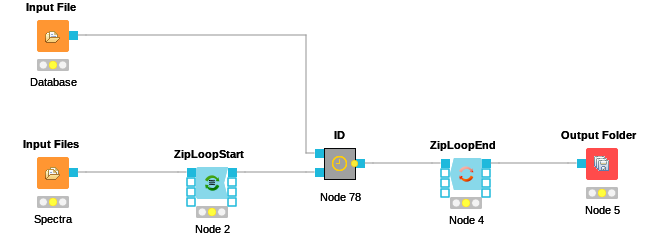
\includegraphics[width=0.59\textwidth]{graphics/knime_basics/workflow}
\caption{The finished supervised learning and prediction workflow.}
\label{fig:workflow}
\end{figure}

\subsection{Summary}
In the previous exercises you learnt how to import data into KNIME, transform it, visualize it and learn a model for predictions on new data. But with over 1000 nodes KNIME has much more to offer. The exercises are only meant as a quick primer on some KNIME nodes and concepts. Feel free to play around with nodes you find in the node repository and their settings. Consult the node description view (available under \menu{View > Node Description}) to find out how to use a node. The KNIME website (\url{http://www.knime.org}) also contains additional information, including blog posts about topics such as Anomaly Detection, Sentiment Analysis, Text Processing and many more.